Ben Trout

2014-12-5

Building, Testing 

\begin{tabular}{|p{5cm}|p{5cm}|}
\hline
Building&
This week me and Matt finished the pat on our robot that grabs the rolling goal. It has a servo motor attached to the back of the robot with an axle hub screwed to the servo. We have two axles hooked together with a brace. The one big axle is pushed through two L brackets so the servo has minimal torque on it as we drive around.  
\\
\hline
Testing&
Last week we basically had our robot ready to test whether or not the spinner can hit balls into the air. This week we got it ready for testing. Alex made a plastic spinner while we finished wiring. Nick, David, and Alex are usually in charge of wiring, but near the end of the week I helped Nick finish it up. We watched a video on how to solder and I helped Nick solder the wires to the motors. This will help us not have to worry about the motor hubs coming off in competition, and will save us room horizontally for the spinners. After all this was done we made some cardboard guides for the balls and taped the ramp down. The testing was successful and we could launch small balls all the way to the ceiling. 
\\
\hline
\end{tabular}

\section*{Building}
The grabber that grabs the goal is all done now. We can’t test it till next week, but for how simple a thing is, I was surprised how many glitches I’d run into. At first I tried have to servo motors so we wouldn’t have to worry about torque being an issue. I soon realized that having two servo motors would work because they’d have to be flipped upside down of each other, and when you flip them they only go down half a bars length not lining up the axles. I quickly scratched this plan and moved onto one servo motor positioned so the axle will be directly down the middle of our back bar. I at first just had the servo attached to the axle, but this would cause too much torque on the servo as we drove around. I attached to L brackets to reduce torque and give the axle stability as it spun. The biggest challenge with this whole process was getting the axle in a position that I could thread it through the holes of the L brackets. There was a lot of switching the servo around and moving L brackets around to position that would potentially work.  

\section*{Testing}
As we finished wiring and building we tested Friday after school. We quickly hit some problems as we started. Our spinner would spin so fast it would shake the whole robot causing our light weight paper ramp to bounce up and get hit by the spinner. We did a quick fix by taping it to the ground, but our final plastic ramp should be heavy enough for this to not happen. This will be a concern though, and we may have to cut our spinner down a little more. Some other problems was our guides for the balls were taped to the ground also, but we’ll be working on a way to attach them to the robot next week. Another problem we encountered was every once in a while the spinner would hit a ball perfectly on the top it would cause the spinner to stop and skip some teeth. We may fix this by putting an encoder on the motor and when it feels irregular force against it, it will stop for a split second allowing the ball to pass through. The final problem we encountered was we couldn’t launch the big balls very high. This was largely do to the fact we had a paper ramp and it would get smashed by the big balls not allowing for quality launch. We think a plastic ramp will fix this, but we’ll need to keep it in mind. The only other small problem we had is big balls have trouble getting under the first intake, but as it spins they can get under. The big balls do get stuck though, and we may have to remake the front intake for more clearance between the axle and ground. 

\begin{center}
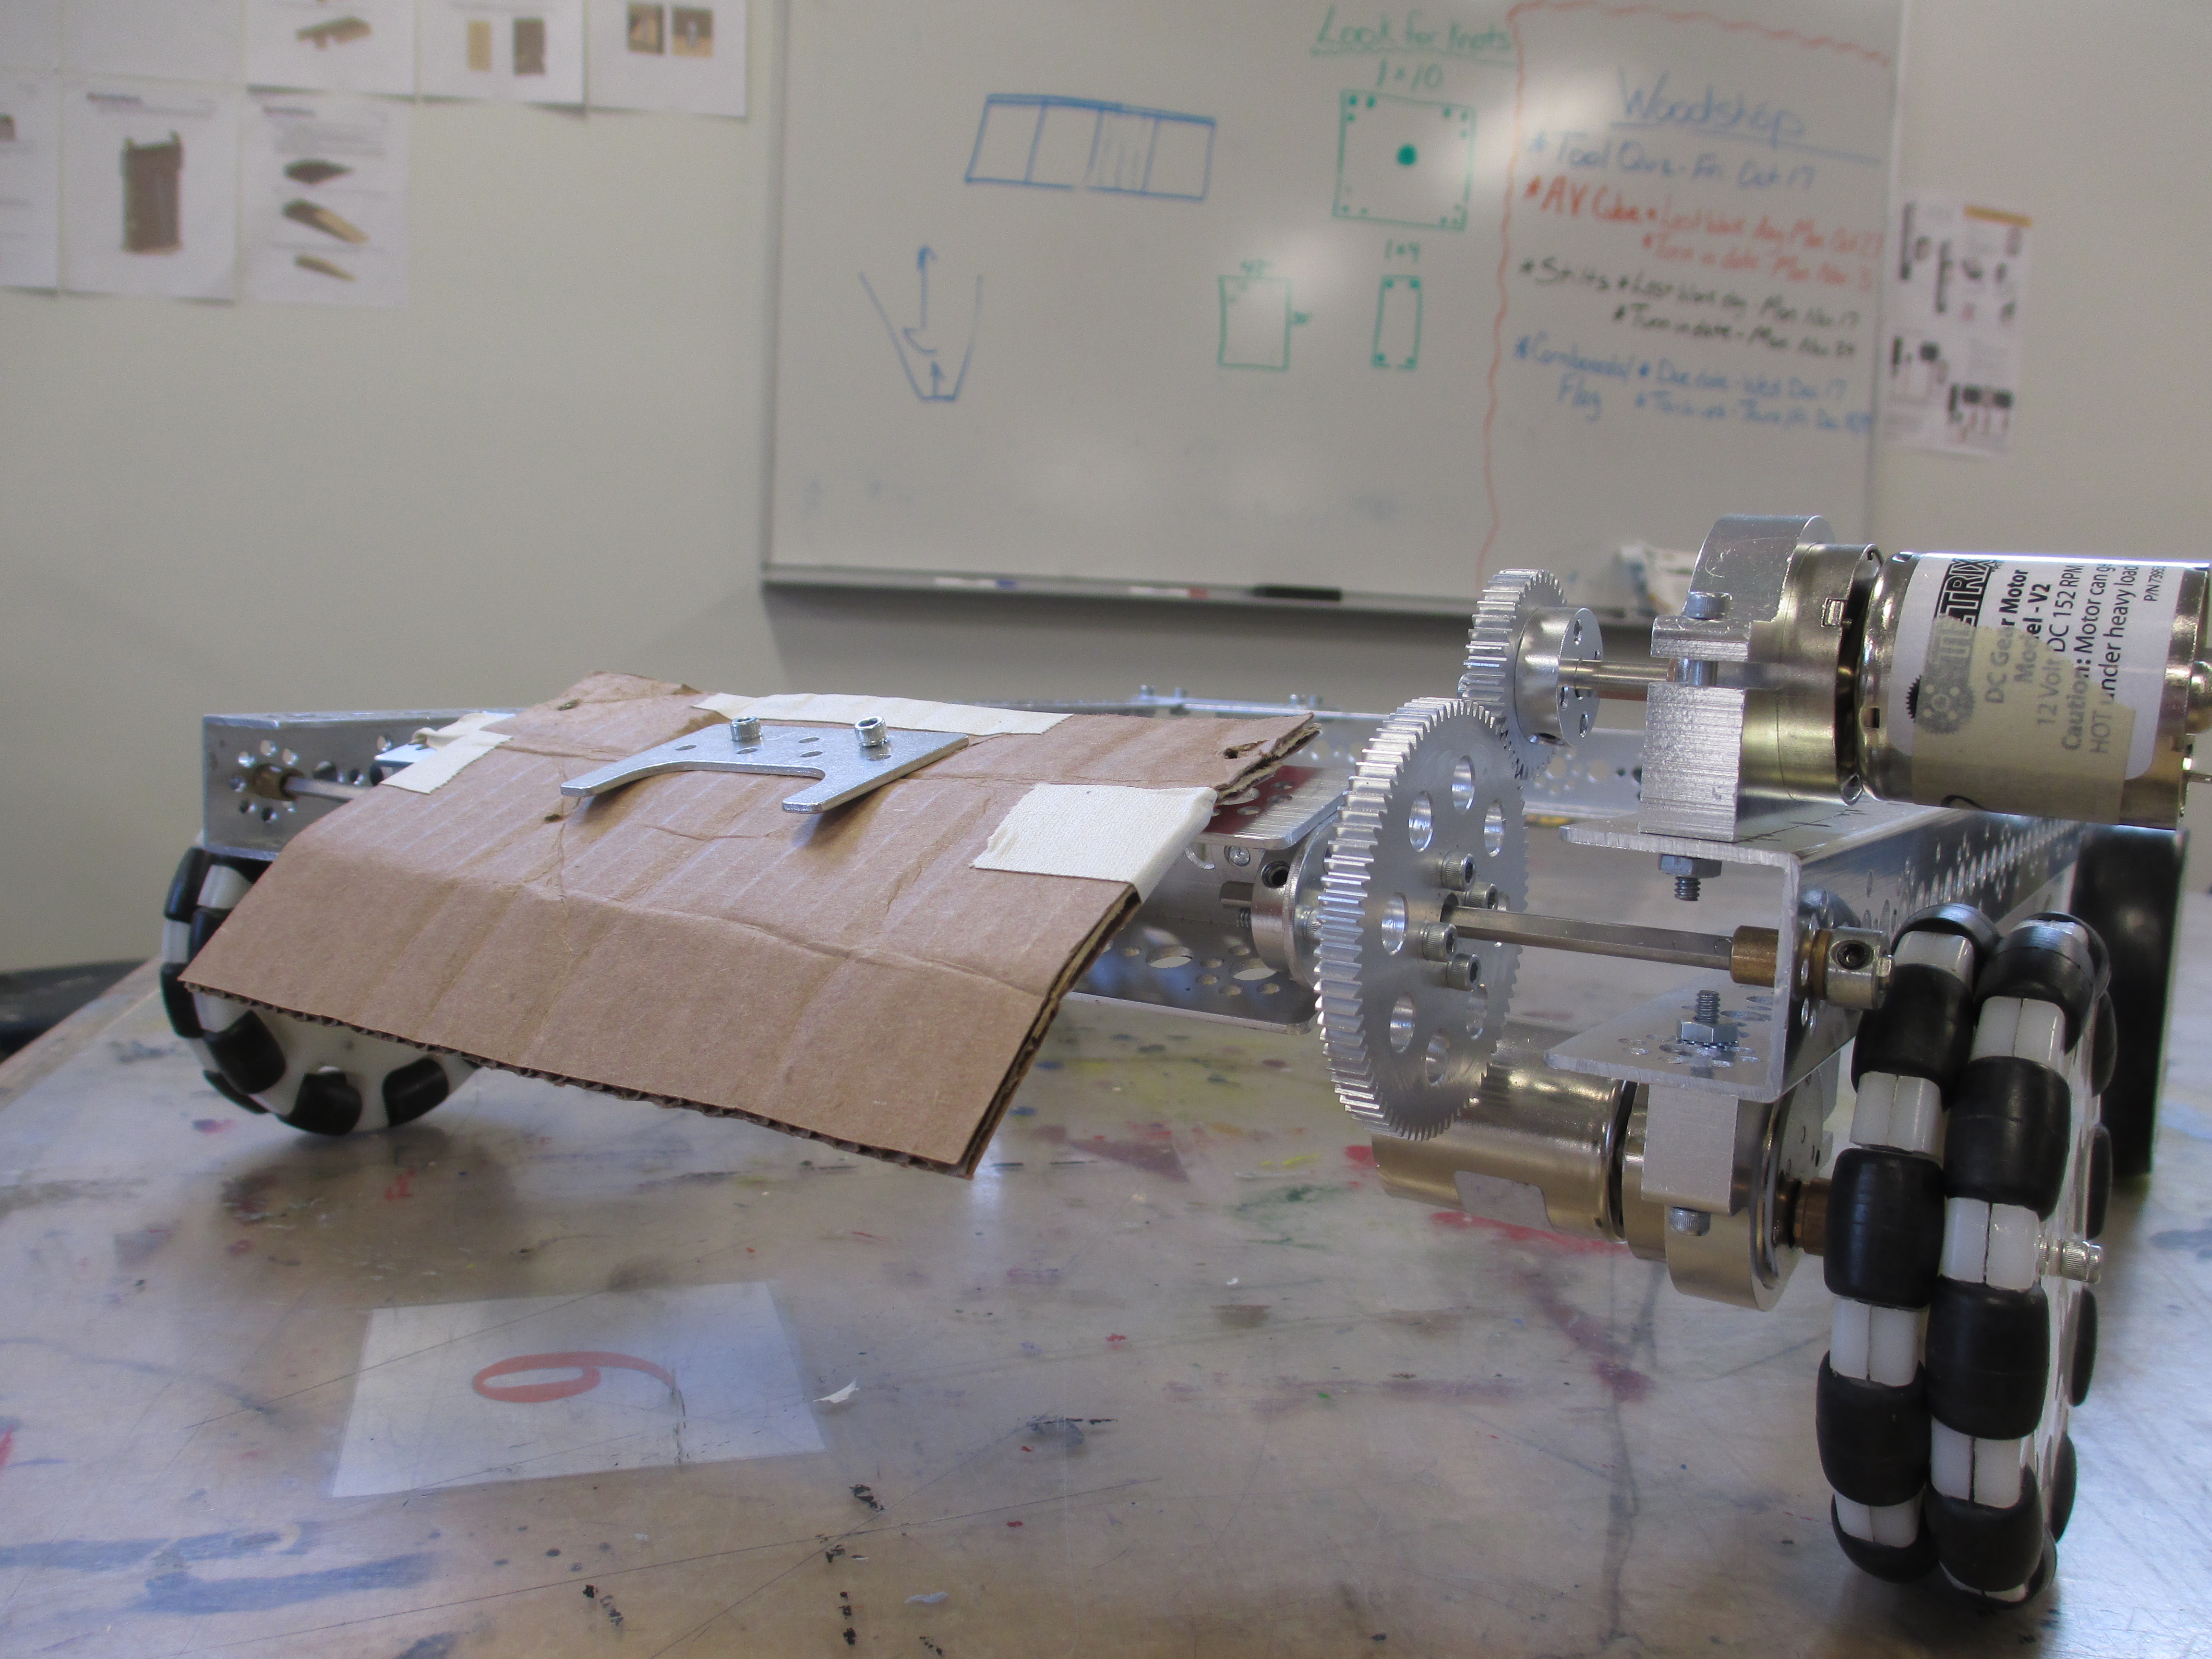
\includegraphics[width=10cm]{./Entries/Images/NewIntake.jpg}
\end{center}
